\documentclass{article}
\usepackage[affil-it]{authblk} % to use the author affiliation tags
\usepackage{graphicx}
\usepackage[space]{grffile}
\usepackage{latexsym}
\usepackage{textcomp}
\usepackage{longtable}
\usepackage{multirow,booktabs}
\usepackage{amsfonts,amsmath,amssymb}
\usepackage{url}
\usepackage{hyperref}
\hypersetup{colorlinks=false,pdfborder={0 0 0}}
\usepackage[utf8]{inputenc}
\usepackage[english]{babel}

\usepackage{natbib}
\bibliographystyle{plainnat}


\begin{document}

\title{Stratospheric ozone intrusion events, characterisation and distribution over high southern latitudes.}

\author[1]{Jesse Greenslade}
\author[2]{Simon Alexander}
\author[3,4]{Robyn Schofield}
\author[1,5]{Jenny Fisher}
\author[2]{Andrew Klekociuk}

\affil[1]{Center for Atmospheric Chemistry, University of Wollongong}
\affil[2]{Australian Antarctic Division, Hobart}
\affil[3]{School of Earth Sciences, University of Melbourne}
\affil[4]{ARC Centre of Excellence for Climate System Science, University of New South Wales}
\affil[5]{School of Earth \& Environmental Sciences, University of Wollongong}

\date{\today}

\bibliographystyle{plain}

\maketitle

\begin{abstract}
  We develop a quantitative method to determine Stratosphere to Troposphere Transport events (STTs) from ozone sonde profiles. 
  Using this method we estimate the quantity of ozone transported across the tropopause over Melbourne ($38^\circ$S), Macquarie Island ($54^\circ$S), and Davis ($69^\circ$S).
  STT seasonality is determined from a 7--9 year long time series of ozone profiles from each site.
  STT events primarily occur during summer above Melbourne and Macquarie Island, while there is little seasonal cycle in STT events above Davis.
  The majority of tropospheric ozone due to STT events occur within 3~km below the tropopause at Melbourne and Macquarie Island, and within 2~km below the tropopause at Davis.
  Overall, the fraction of total tropospheric ozone attributed to STT events is 2 – 4\% at each site, however, during individual events, an STT event can contribute more than 10\% of the total tropospheric ozone at that time.
  TODO:We also need to note favourable or unfavourable comparisons between our ozone flux results and previous model\/obs studies; also a sentence about GEOS-Chem results.
\end{abstract}%


\section{Introduction}

    %\subsection{Background}
    Tropospheric ozone, which constitutes only 10\% of the total ozone column, is an important oxidant, greenhouse gas and is toxic to biological life. 
    Over the industrial period, increasing tropospheric ozone, has been estimated to exert a radiative forcing equivalent to a quarter of the CO$_2$ forcing \citep{IPCC_Chapter2}. Tropospheric ozone increases above pre-industrial levels are estimated to result in global losses up to \$USD$_{2000}$ 35 billion per annum until 2030 due to food crop impacts \citep{Avnery2011} and up to \$USD$_{2000}$ 580 billion by 2050 (~11.8 billion per year) due to health impacts \citep{Selin2009}. Tropospheric ozone is produced anthropogenically by fossil fuel and biomass combustion emissions (NO$_x$ and volatile organic compounds) that subsequently undergo photochemistry. Natural sources of tropospheric ozone include the downward transport from the ozone-rich stratosphere, wildfires and lightning photochemical production (\citet{Jacobsonsxxxx}Jacobson and references therein). 
 
    Stratosphere to troposphere transport (STT) of ozone can increase regional surface ozone levels above air quality standard thresholds \citep{Danielson1968, Lefohn2011, Langford2012, Zhang2014}. A review of photochemical models by \citet{Stohl2003} (STACCATO) concluded that between 25-50\% of tropospheric ozone can be attributed to SST events. A lower estimate was derived from the Atmospheric Chemistry and Climate Model Intercomparison Project (ACCMIP), \citet{Stevenson2006} with $5100\pm600$ Tg/yr (\~90\%) and $550\pm170$ Tg/yr (\~10\%) of tropospheric ozone is due to chemical production and STT, respectively. Models are challenged to correctly represent STT, and process studies seem to be key in determining the relative role of SST in the tropospheric ozone budget.
    
    STT events have been observed due to deep overshooting convection \citep{Frey2015}, tropical cyclones \citep{Das2016} and mid-latitude synoptic scale disturbances (e.g. \citet{Stohl2003,Mihalikova2012}). STT events observed over the Mediterranian region estimate a 10\% contribution to tropospheric ozone budget between 2000 and 2003 \citep{Galani2003}, with other observational studies noting significant occurrences and strong seasonal dependance (i.e. \citet{Lefohn2011}), contributing up to 30\% of the surface ozone over the Western US in spring \citep{Lin2012}. To date, while this topic has received significant attention in the tropics and northern hemisphere, observational estimates from the southern hemisphere extra-tropics is noticeably absent in the literature. 
    
    In the extra-tropics, ozone has a longer photochemical lifetime and STT events most commonly occur during synoptic-scale tropopause folds \citep{Sprenger2003, Tang2012} which are characterised by tongues of high Potential Vorticity (PV) air descending to low altitudes. These tongues become elongated and filaments disperse away from the tongue and mix irreversibly into the troposphere. STT events have been observed in tropopause folds around both the polar-front jet \citep{Vaughan1994, Beekmann1997}, and the subtropical jet \citep{Baray2000} and cut-off lows \citep{Price1993, Wirth1995}.  A high correlation is found between lower stratospheric and tropospheric ozone \citep{Terao2008} with the highest STT associated with jet-streams over the oceans in winter.
  
 %Move to discussion / conclusion ... \citet{Hegglin_2009} estimate that climate change will lead to increased STT of the order of 30 (121) Tg yr$^{-1}$ relative to 1965 in the Southern (Northern) Hemisphere due to an acceleration in the Brewer Dobson circulation. Tropospheric ozone is lost via chemical destruction and dry deposition, estimated to be $4700\pm700$ Tg/yr and $1000\pm200$ Tg/yr, respectively \citep{Stevenson2006}. 

    %Hegglin, M. I., and T. G. Shepherd (2009), Large climate-induced changes in ultraviolet index and stratosphere-to-troposphere ozone flux, Nature Geosci, 2(10), 687–\selectlanguage{english}691, doi:10.1038/NGEO604.

    % AIMs paragraph
    In section 2 we use several years of ozonesonde flights from three locations spanning the 38$^{\circ}$S - 69$^{\circ}$S latitudes to characterise the seasonal cycle of STT events and determine their contribution to the total amount of tropospheric ozone.
    We examine the depth and frequency of the intrusions and use case studies to relate these STTs to meteorological events.
    Lastly, we calculate the fraction of total tropospheric column ozone attributed to STT events.

\section{Data and Methods}

  \subsection{Ozonesonde record in the Southern Ocean}
    Ozonesondes are weather balloons with an attached instrument which measures ozone concentrations roughly every 100m from the surface to around 35km.
    These ozonesondes provide a high-vertical resolution profile of ozone, along with temperature, pressure, and humidity.
    
    Ozonesondes use an electrochemical concentration cell which senses the proportional electrical current from ozone's reaction to a solution of potassium iodide.
    Each ozonesonde is completely new and independant, so calibration is replaced by following standardised procedures when creating, transporting, and releasing them.
    Ozonesondes are estimated to provide around 2\% precision in the stratosphere, with increasing precision at lower altitudes \citep{noaasondes}, although the accuracy has been shown to be around 5-10\% which gets worse if standardised procedures aren't followed \citep{Smit2007}.
    
    Ozonesondes are launched approximately weekly from Melbourne (38$^{\circ}$S, 145$^{\circ}$E), Macquarie Island (55$^{\circ}$S, 159$^{\circ}$E) and Davis (69$^{\circ}$S, 78$^{\circ}$E). 
    For this study, we use the data collected from 2004-2013 for Melbourne and Macquarie, and 2006-2013 for Davis. 
    Around twice as many ozonesonde launches occur at Davis prior to and during the ozone hole season (June-October) than at other times of the year \citep{Alexander2013}.
    
    %The ERA-I data we used for synoptic weather was of one degree horizontal resolution with pressure levels at 200, 300, 400, and 500 hPa.
    %For individual cases ERA-I data was downloaded at .25 degree horizontal resolution with the full 34 pressure levels from 1000 to 1 hPa. 

  \subsection{Characterisation of STT events and associated fluxes}
    \label{Section:CharacterisationOfSTTs}
    
    Stratospheric ozone typically mixes irreversibly down (vertically) into the troposphere in kilometres-scale tongues of air.
    The altitude of the tropospheric ozone peak due to an STT event and the amplitude of the event above the background tropospheric ozone profile vary in space and time.
    While ozone sondes are released every week or so, ozone events may only be detectable for a matter of hours \citep{Tang2012}.
    The vertical ozone profile recorded by the ozonesonde is highly dependent on the time of launch \citep{Sprenger2003}, and we cannot guarantee that detected ozone enhancements are fully separated from the stratosphere.
    
    In order to characterise tropospheric ozone events a clear definition of where the stratosphere begins is necessary.
    Tropopause height can be defined based on the standard lapse rate tropopause \citep{WMO1957} or the ozone tropopause \citep{Bethan1996}.
    The lapse rate is the negative altitudinal temperature gradient, while the lapse rate tropopause is defined as the lowest altitude where the lapse rate is below 2$^\circ$~C~$km^{-1}$, provided the lapse rate between this altitude and all subsequent altitudes within 2~km is also below 2$^\circ$~C~$km^{-1}$.
    The ozone tropopause is defined as the lowest altitude satisfying these three conditions \citep{Bethan1996}:
    \begin{enumerate}
      \item Vertical gradient of ozone mixing ratio (OMR) is greater than 60~ppbv km$^{-1}$
      \item OMR is greater than 80~ppbv
      \item OMR between 500~m and 2000~m (1500~m in the Antarctic) above exceeds 110~ppbv.
    \end{enumerate}
    At Davis, the ozone tropopause defintion is modified since the site is Antarctic.
    While the ozone tropopause can be less robust during stratosphere-troposphere exchange, it performs better than the lapse rate tropopause at polar latitudes in winter and near jet streams in the lower stratosphere \citep{Bethan1996, Tomikawa2009, Alexander2013}. 
    We use the lower of these two tropopause altitudes for this study.
    This choice avoids occasional unrealistically high tropopause heights due to perturbed ozone or temperature measurements in ozonesonde records.
    
    Figure \ref{fig:seasonaltpheights} shows the monthly mean tropopause altitudes at each location, along with the subset of altitudes from profiles for which an STT event was determined. 
    The seasonal cycle in tropopause altitude at Melbourne is clearly apparent, as is the decreasing tropopause altitude which occurs at higher southern latitudes.
    The tropopause recorded by sonde is generally higher during an STT event at all three sites.
    Tropopause altitudes at Davis may exceed 11~km altitude under certain synoptic conditions \citep{Alexander2013}; the relation of tropopause altitude with individual STT events is investigated in detail below.

    \begin{figure}[!htbp]
	\begin{center}
	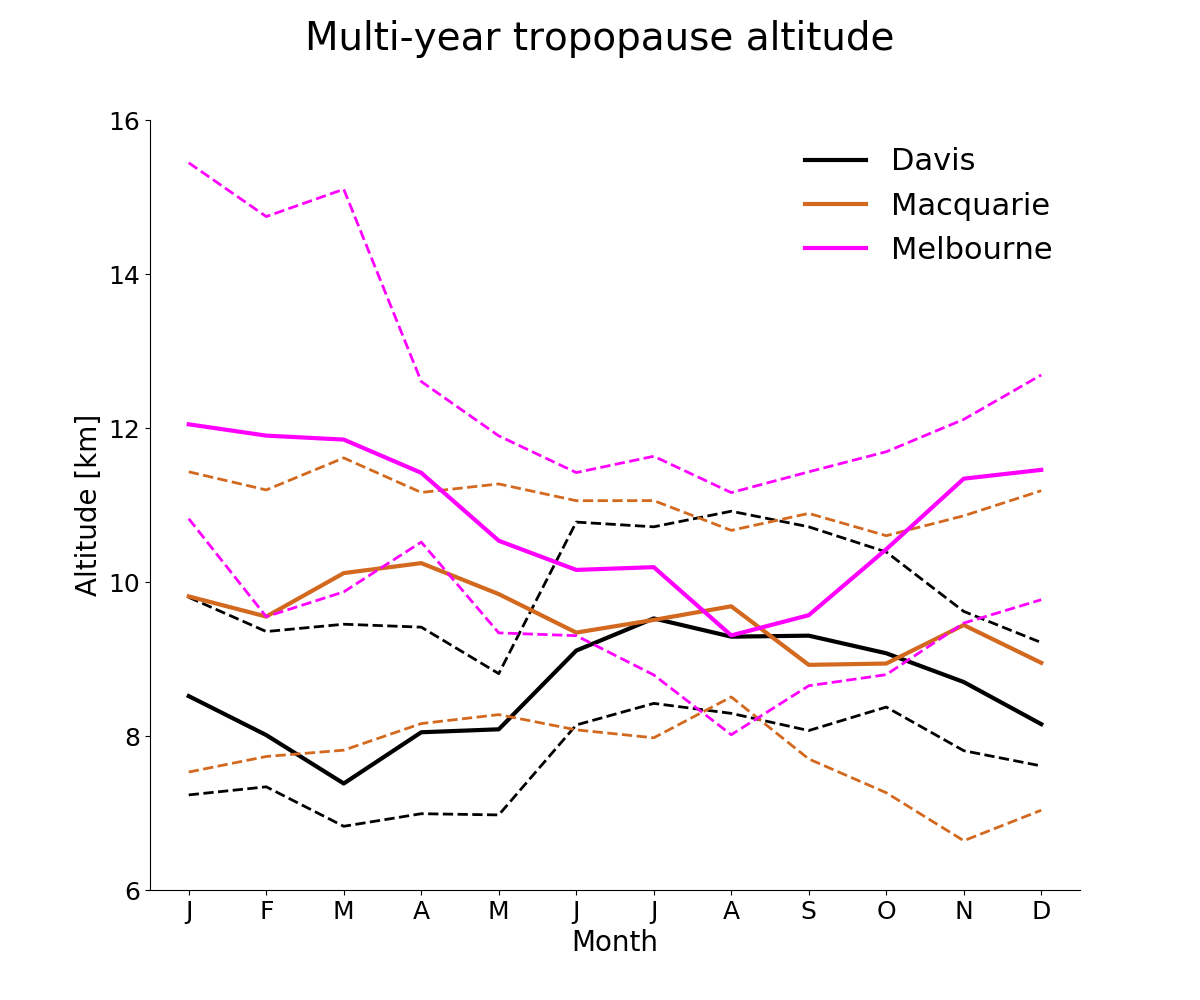
\includegraphics[width=0.8\columnwidth]{figures/tpheights}
	\caption{Monthly mean tropopause altitudes (minimum of lapse-rate and ozone defined tropopause at 3 sites) determined from ozone sondes.
	Dashed lines show the average monthly altitude when only considering dates when STTs occured.) 
	}
	\label{fig:seasonaltpheights}
	\end{center}
    \end{figure}

    Figure \ref{fig:seasonaltropozone} shows seasonally averaged ozone as recorded over the three stations.
    Increased ozone extending down through the stratosphere is apparent during December to March and September to November over Melbourne.
    These increased tropospheric ozone months are due to STTs (in summer), and possible fire smoke plume influence (in winter).
    Over Davis and Macquarie Island the tropospheric ozone is higher between March and October, although the effect is subtle compared to Melbourne.
    
    \begin{figure}[!htbp]
      \begin{center}
      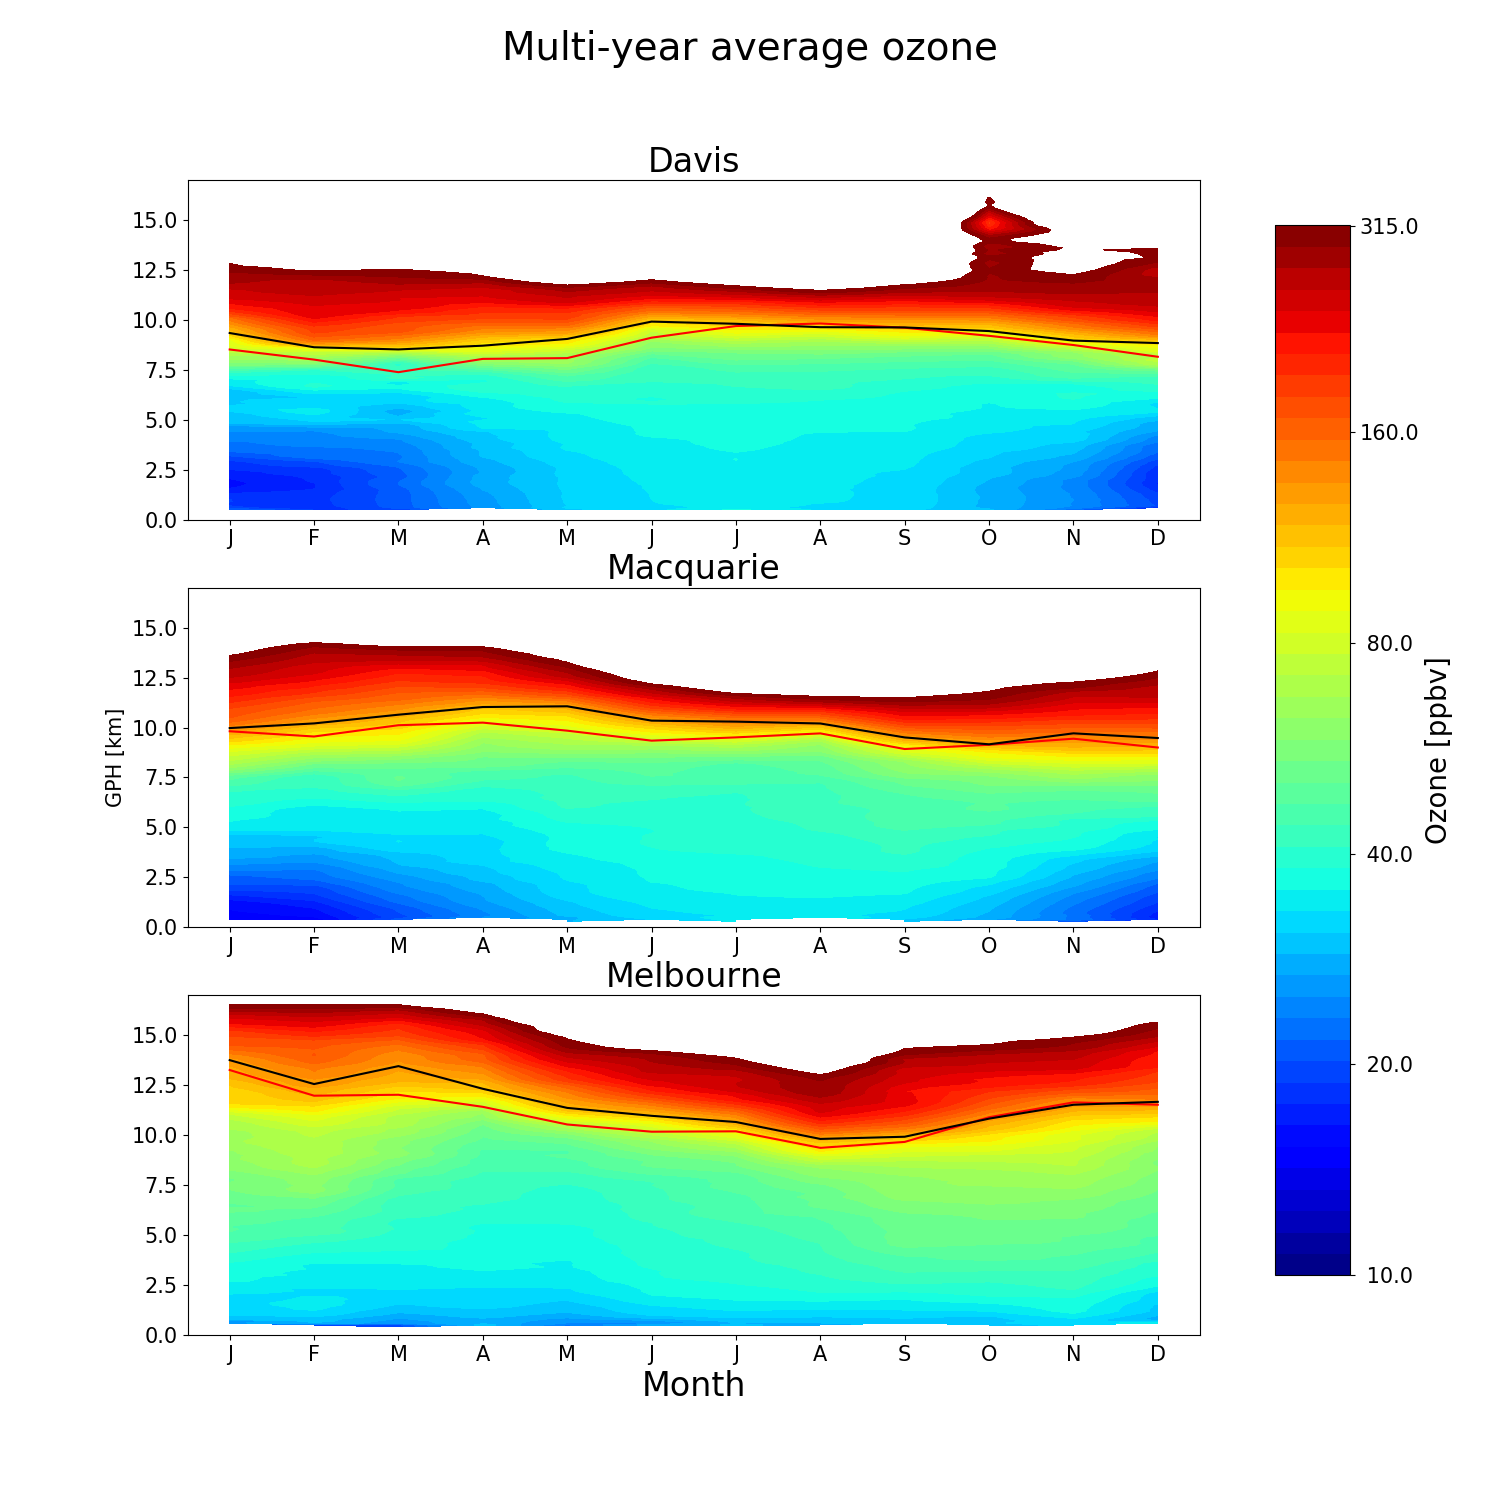
\includegraphics[width=0.8\columnwidth]{figures/seasonaltropozone}
      \caption{
      Seasonal cycle of ozone over Davis, Macquarie, and Melbourne measured by ozonesondes, where measurements are binned monthly.
      Black solid lines show seasonal tropopause heights, defined as described in the text.
      }
      \label{fig:seasonaltropozone}
      \end{center}
    \end{figure}
    
    %One important factor of STT characterisation was the height of the tropopause, which can be defined in several ways.
    %Using only the ozonesonde datasets, the tropopause from ozone and lapse rate definitions are easy to calculate.
    %While the ozone tropopause can be less robust during stratosphere-troposphere exchange, it performs better than the lapse rate tropopause at polar latitudes in winter and near jet streams in the lower stratosphere \citep{Bethan1996}.
    %For many of the sonde profiles ozone disturbances occur between the lapse rate and ozone defined tropopauses, and since it is not clear that this area is actually the troposphere we only characterise events bound by the lower of the lapse rate and ozone tropopause heights.

    \citet{Tang2010} define one method of detecting these stratospheric tongues (or tropospheric ozone folds)  as follows: From 5~km altitude, if the ozone level exceeds 80~ppb and then within 3~km decreases by 20~ppb or more to a value less than 120~ppb, then a tropopause fold has occurred.
    Their definition is based on subjective analysis of sondes released from 20 stations in the latitudinal range from 35$^\circ$S to 40$^\circ$N.
    We also characterise STT events using the ozonesondes vertical profiles, looking for tropospheric ozone enhancement above a local background (in moles per billion moles of air, or ppb).
    In this paper we define tropospheric ozone events based on a subjective analysis of ozonesonde profiles at three sites at 38$^\circ$S, 55$^\circ$S, and 69$^\circ$S.
    
    TODO: More of simon's changes here, clarify analysis and sensitivity
    To identify STT events, the vertical profiles of ozone volume mixing ratio are linearly interpolated to a regular grid with 20~m resolution up to 14~km altitude and are then bandpass filtered to retain perturbations with vertical scales between 0.5~km and 5~km.
    From here onwards the filtered vertical profile is referred to as the perturbation profile.
    The choice of band limits was set empirically; for an event to qualify as STT, a clear increase above the background ozone level is needed, and a vertical limit of $\sim 5$~km removes seasonal-scale effects.
    We exclude from analysis perturbations at altitudes below 4~km above the surface to avoid surface pollution events and those occuring within 0.5~km of the tropopause to avoid the sharp transition to stratospheric air producing spurious false positives.
    Then using ozone perturbations from 2~km above the surface up to 1~km below the tropopause, we create a threshhold for each launch site at the 99th percentile.
    Profiles with perturbations exceeding this threshhold are initially classified as STT events.
    
    The ozone peak is defined at the altitude where the OMR is greatest within the lowest range of altitudes where the perturbation profile exceeds the percentile based threshhold.
    If the OMR between this ozone peak and the tropopause drop below 80~ppb and are more than 20~ppb lower than the peak ozone then the initially classified event is confirmed, otherwise the profile is rejected as a non-event.
    This confirmation is only required if the perturbation profile does not drop below zero between the event peak and the tropopause.
    This happens in order to remove `near tropopause' anomalies for which there is no evidence of detachment from the stratosphere.

    We conservatively estimate the ozone flux into the troposphere associated with each event.
    The estimate is conservative since it does not take into any secondary ozone enhancements which may have been caused by the STT, as well as ignoring any heightened ozone background levels which may be due to synoptic-scale stratospheric mixing into the troposphere.
    The ozone concentration is integrated vertically over the altitude range for which an STT event is identified.
    Figure~\ref{fig:filterEG} shows an example ozone profile, and how the algorithm detects an STT event, defines the event boundaries, and calculates the ozone flux.
    
    \begin{figure}[!htbp]
      % Figure created in getevents.pro, edited in inkscape
      \begin{center}
      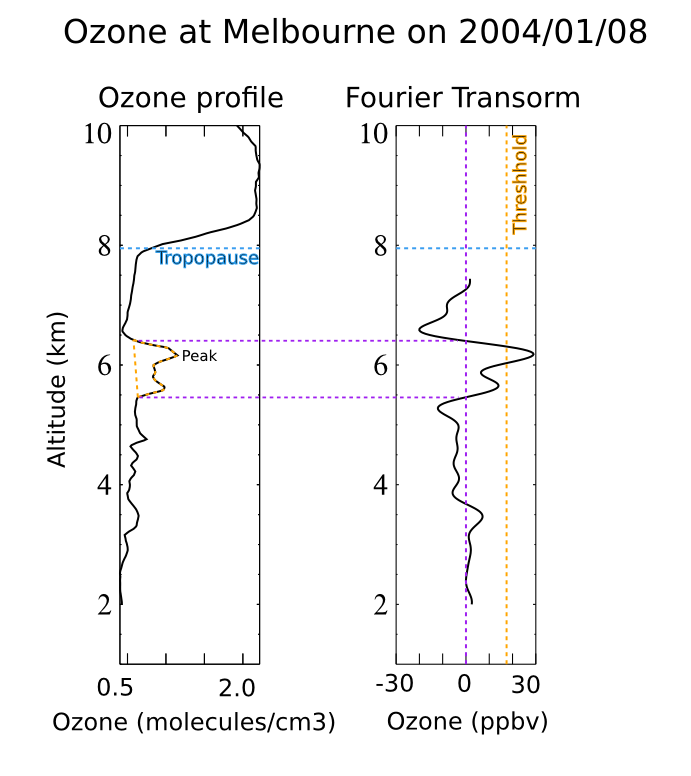
\includegraphics[width=0.8\columnwidth]{figures/filtereg.png}
      \caption{ Left: an example illustrating methods used for STT identification and flux estimation using an ozone profile from 2km to the tropopause (dashed vertical line).
      At Melbourne on the 8th of January 2004 the flux area shows the estimate of stratospheric impact on tropospheric ozone.
      Right: band pass filtered O$_3$ ppb perturbation profile.
      Coloured lines show the 99th percentile of filtered ozone perturbations (purple dashed) and the technique for determining the vertical extent of the event (orange dashed) is outlined in the text.
      See text for details.
      }
      \label{fig:filterEG}
      \end{center}
    \end{figure}

  \subsection{Sensitivities and limitations}
    There are several observationally defined threshholds and limits which have an effect on how many events are detected, what altitude within which they can be detected, and how strongly the events are separated from the stratosphere.
    
    The cutoff threshhold (defined locally to each site) is determined from the 99th percentile of the filtered ozone profile between 2~km and the tropopause height minus 1 kilometer.
    If an ozonesonde's filtered profile (between 4~km and the tropopause minus 500~m) goes above this threshhold then the profile is flagged as an event.
    Changing either of these altitude ranges, or the cutoff threshhold, changes how many events are detected.
    For example, using the 98.5th percentile increased detected events by 26 and Melbourne, 18 at Macquarie Island, and 9 at Davis.
    We use the 99th percentile because at this point the filter locates clear events with no obvious false positives.
    
    The altitude range for flagging filtered profiles is set from 4~km above the surface to 500~m below the tropopause .
    This range removes possible ground pollution effects as well as local fire smoke plumes which are not likely to ascend above 4~km, as well as allowing event detection up to 500~m from the tropopause.
    Some events, including the storm-caused event examined in figure \ref{fig:Melbourne20050203} are within one kilometer of the tropopause. 
    
    The altitude range used to determine the 99th percentile is set from 2~km up to 1~km below the tropopause.
    This range removes any anomalous edge effects of the Fourier filter, as well as discounting the highly variable ozone concentration which occurs near the tropopause.
    
  \subsection{Removal of biomass burning influence}
    
    Other sources of tropospheric ozone profile perturbation need to be analysed and excluded before drawing any conclusions about STTs based on recorded ozone profiles. 
    The major possible ozone influence other than STTs in the troposphere above 4~km is smoke plumes from biomass burning.
    
    Ozone production from biomass burning is complex and affected by photochemistry, fuel nitrogen load, time since emission, and atmospheric plume chemistry both during transport and at the point of measurement.
    %Ozone precursors include nitrogen oxides ($NO_x = NO + NO_2$) and non methane volatile organic compounds (NMVOCs). % too basic for here..
    Large biomass burning events emit substantial ozone precursors, some of which are capable of being transported far from their origins. 
    Peroxyacetyl Nitrate (PAN) is a reservoir of NO$_x$ which can lead to enhanced ozone far from the source of a fire \citep{Jaffe_2012}.
    
    Biomass burning influence in the Southern Hemisphere comes mostly from Southern Africa and South America, however Australian fires from the midlatitudes, and Indonesian fires can also influence the ozonesonde release sites.
    Transported biomass burning plumes influence the southern mid-latitudes generally between July and December \citep{Pak2003}.
    Biomass burning smoke plumes can lead to enhanced ozone, however this is not always the case.
    Due to the possible influence of smoke plumes on identification of STT events we exclude from analysis any dates where they are seen near the ozonesonde launch sites.
    
    Removal of any possible influence from biomass burning smoke plumes is performed by detection of smoke plumes through global CO measurements.
    Here we identify transported smoke plumes through enhanced carbon monoxide (CO) levels.
    CO has a long enough lifetime to be an effective tracer of transport.
    The primary source of atmospheric enhancement of CO is fires, making CO a good indicator of fire plumes.
    Using high CO levels as a proxy for smoke plumes is a well established method (eg: \citet{Edwards2003,Sinha2004,Edwards2006,Mari2008}).
    We use data from the AIRS (Atmospheric Infrared Sounder) instrument on board the Aqua satellite \citep{AIRS3STD}.
    We visually inspect AIRS' vertical columns of CO over the Southern Hemisphere to exclude events with possible smoke influence at our three sites.
    We diagnose smoke plumes where high ($\approx 2 \times 10^{18}$ molecules cm$^{-2}$ or higher) CO columns appear and when these occur near our sites during a sonde-detected ozone event we remove the event from STT analysis.

    Figure \ref{fig:excludedeg}(top) shows a day where smoke plumes are near the Melbourne sonde launch site on the day of a detected event. 
    An event preliminarily detected on this day through the ozonesonde data is flagged as possibly due to fire.
    In the figure elevated CO levels can be seen over Australia, likely due to long-range transport from African and/or South American biomass burning.
    This day can be contrasted with the example in figure \ref{fig:excludedeg}(bottom) where low CO levels are observed over the entire Southern Hemisphere.
    We screened all days at all three sites where an STT event is detected except for one event that coincided with missing AIRS data (January 2010). 
    We flagged 15 of 72 events over Melbourne, 8 of 48 events over Macquarie island, and none from 45 over Davis.
    Nearly all of the discarded events occur within the burning season of the Southern Hemisphere.
    
    \begin{figure}[!htbp]
      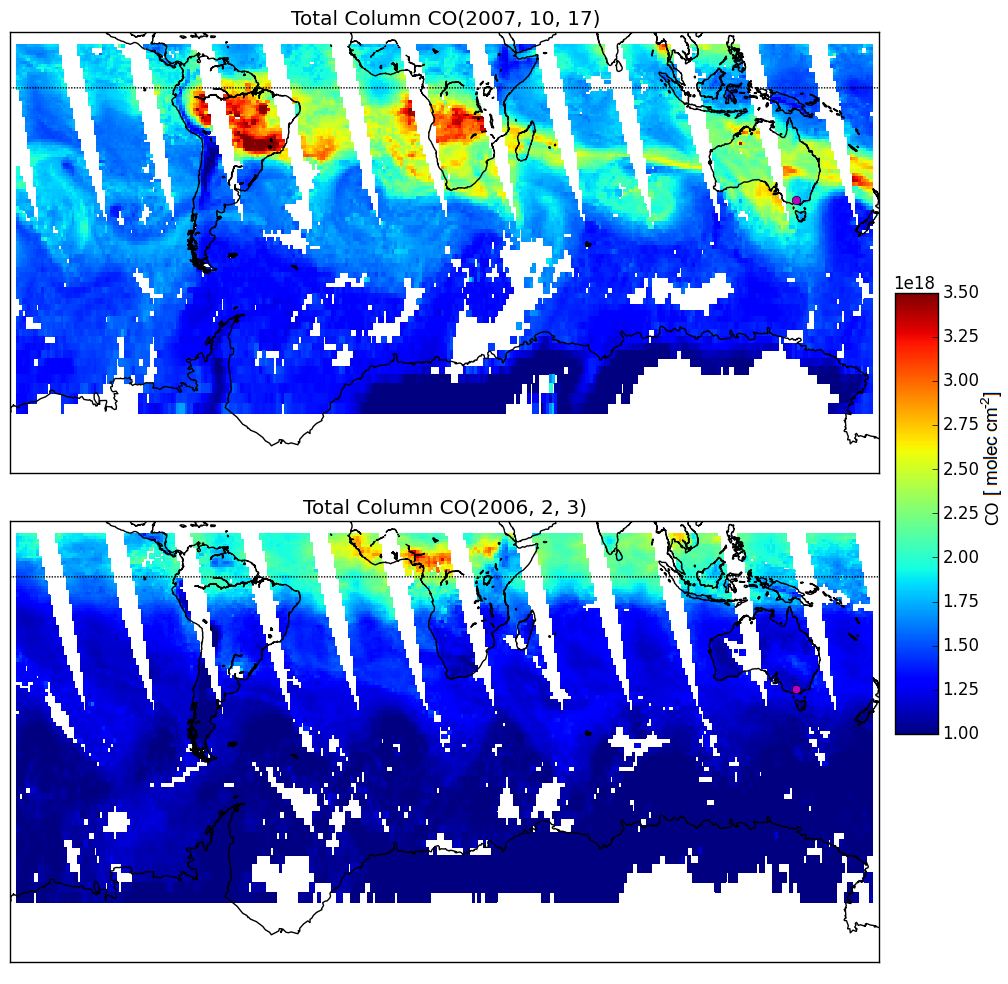
\includegraphics[width=\textwidth]{figures/AIRS_compare.png}
      \caption{AIRS total column CO.
      The top panel (17 October 2007) is a day when ozone above Melbourne (purple dot) could have been caused by a transported biomass burning plume, and so was excluded from analysis.
      The bottom panel (3 February 2006) shows an example of a day when Melbourne ozone was likely not influenced by transported smoke plumes and was retained for analysis.}
      \label{fig:excludedeg}
    \end{figure}
    
    We also include on Figure~\ref{fig:SummarySeasonality} to Figure~\ref{fig:SummaryTPDepths} the events which have possible fire influence. 
    These events are concentrated in spring at Melbourne and Macquarie Island.

\section{Case Studies of synoptic conditions during STT events}

  We examine two case studies in detail to illustrate the synoptic-scale conditions in which STT events occur over Melbourne.
  Data from the European Center for Medium-range Weather Forecasts (ECMWF) Interim Reanalysis (ERA-I) \citep{Dee2011} product is used for synoptic-scale examination of weather patterns over our three sites on dates matching detected STT events.
  
  Figure \ref{fig:Melbourne20050203}(left) shows the ozonesonde profile recorded on the 3rd of February 2005 above Melbourne.
  Both tropopause definitions are between 400 and 500 hPa and the ozone spikes have clear anticorrelations with the relative humidity, suggesting dry stratospheric air is measured here. 
  An ozone intrusion into the troposphere is identified by our detection algorithm at $\sim520$~hPa.
  Figure \ref{fig:Melbourne20050203}(right) shows the synoptic weather system, a cut-off low pressure system which caused a large storm and lowered the local tropopause height for several days.
  The wind circles around the low pressure system in a clockwise direction, typical geostrophic flows which are caused by pressure gradients and coriolis forces.
  The flux of stratospheric ozone brought into the troposphere by this event is at least $3.1 \times 10^{11}$ molecules cm$^{-3}$ , or 8\% of the tropospheric ozone column.

  \begin{figure}[!htbp]
  % these IMAGE CREATED BY show_profile.py, EDITTED IN INKSCAPE
    \begin{center}
    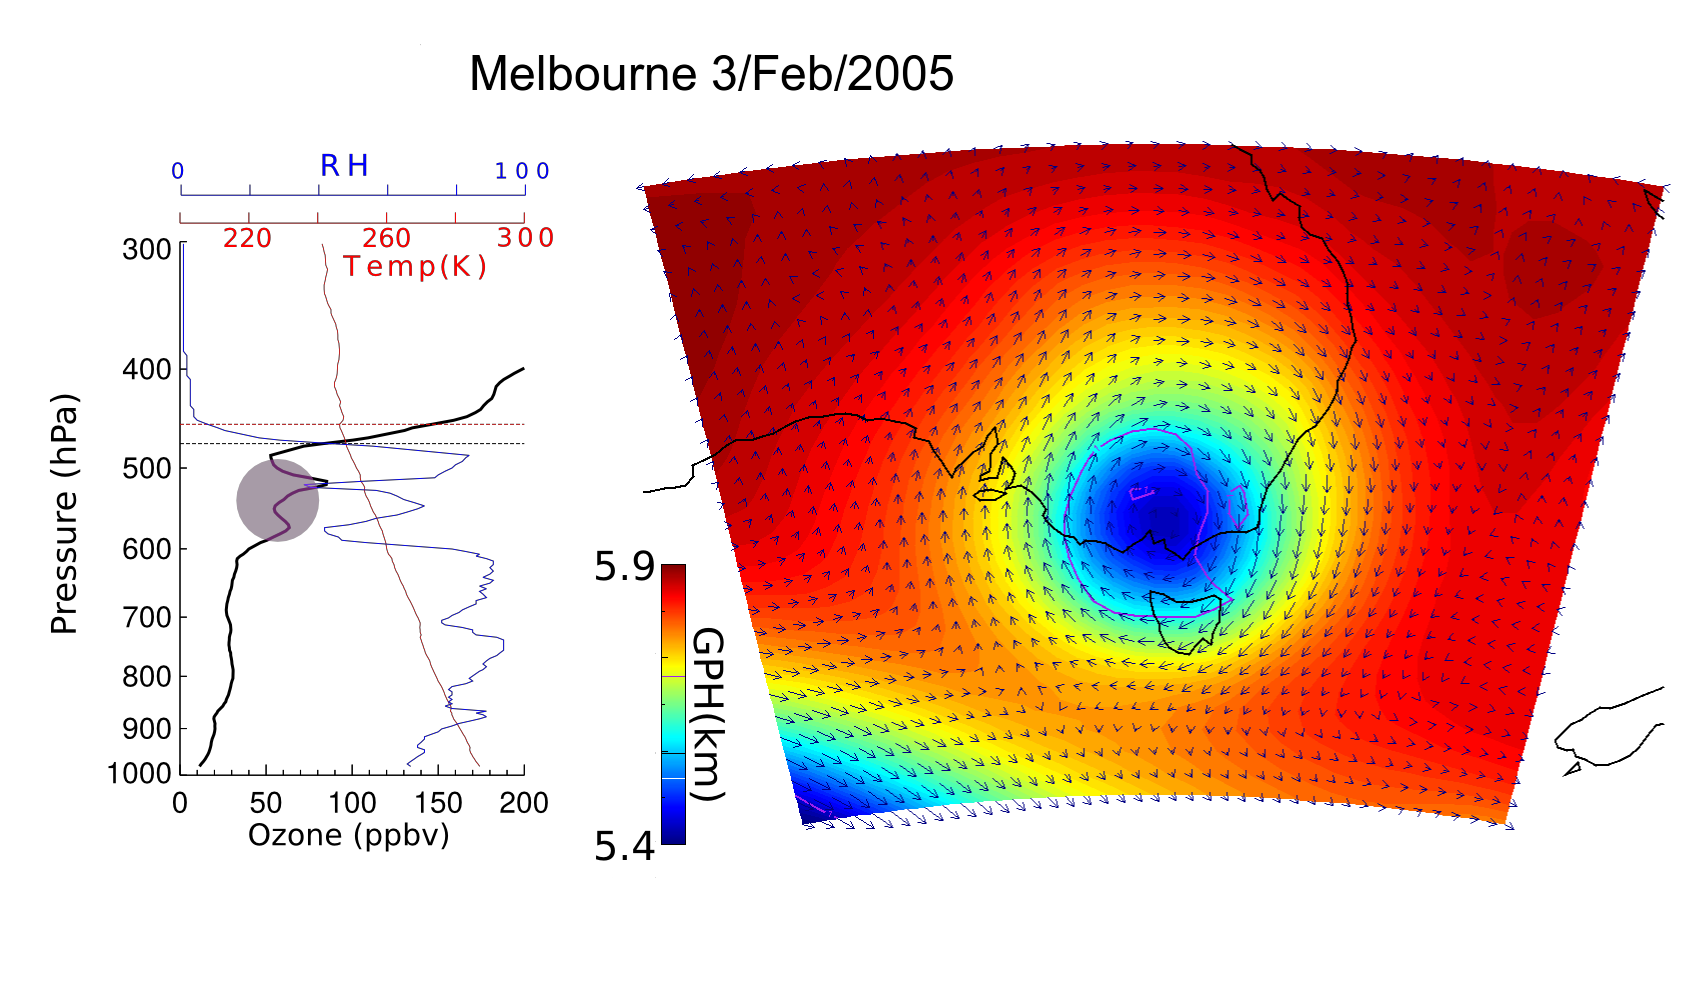
\includegraphics[width=1.0\columnwidth]{figures/Melbourne20050203.png}
    \caption{(Left) Vertical profile of ozone (black line), relative humidity (blue line), and temperature (red line) for  3 February 2005.
    The STT ozone event is highlighted in pink.
    The tropopause heights using both the ozone definition (black dashed line) and lapse rate definition (red dashed line) are shown.
    (Right) Synoptic weather map at 500 hPa from the ERA-Interim reanalysis.
    Vectors show wind direction and speed while colour indicates the geopotential height.
    Also visible are contours of potential vorticity units with 1 PVU in purple and 2 PVU (often used to determine dynamical tropopause height) in white.}
    \label{fig:Melbourne20050203}
    \end{center}
  \end{figure}
  
  Figure \ref{fig:Melbourne20100113}(left) shows the vertical ozonesonde profile recorded on the 13th January 2010 over Melbourne.
  The tropopause heights are greater at this time and an ozone intrusion is identified centred around 200~hPa.
  Again, anticorrelated relative humidity provides evidence that the air is stratospheric in origin.
  Note the separation between this intrusion and the ozone tropopause (marked by the black dashed line), which indicates that the sonde passes through regular tropospheric air after hitting a stratospheric intrusion but before reaching the tropopause.
  Figure \ref{fig:Melbourne20100113}(right) shows a trough of low pressure (front) passing over south-eastern Australia.
  This low pressure system crosses west to east and causes a wave of lowered tropopause height, which is often the cause of stratospheric mixing.
  During frontal passage, stratospheric air descends and streamers of ozone-rich air break off and mix into the troposphere \citep{Sprenger2003}.
  
  \begin{figure}[!htbp]
  % these IMAGE CREATED BY show_profile.py, EDITTED IN INKSCAPE
    \begin{center}
    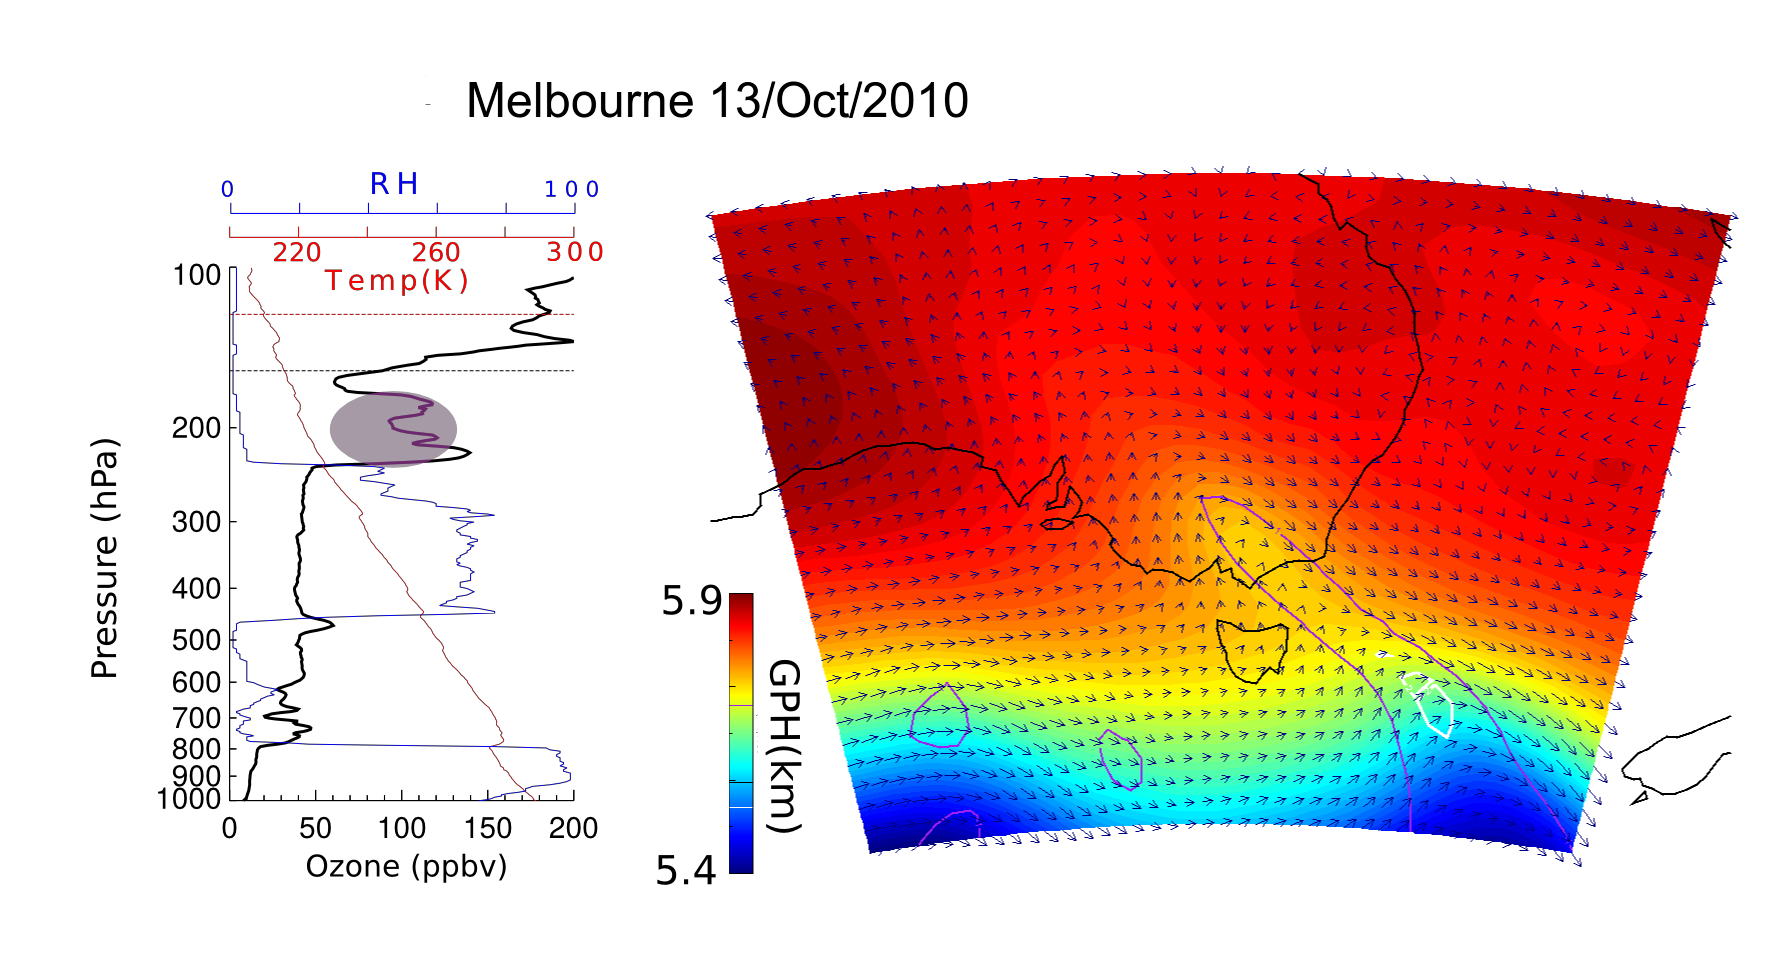
\includegraphics[width=1.0\columnwidth]{figures/Melbourne20100113.png}
    \caption{As figure \ref{fig:Melbourne20050203}, for 13 January 2010.}
    \label{fig:Melbourne20100113}
    \end{center}
  \end{figure}

  We investigate other STT events above Melbourne, Macquarie Island, and Davis, using reanalysis data.
  Similar characteristics to the case studies presented here occur over Macquarie Island: i.e. a prevalence of frontal and low pressure activity during STT events.
  Typically during STT occurrence, the upper troposphere is not calm, with low pressure fronts or cut-offs nearby at coincident time.
  Over Davis the weather systems are harder to distinguish, and the polar vortex may create ozone folds without other sources of upper tropospheric turbulence.

\section{STT event climatologies}

  Figure \ref{fig:SummarySeasonality} shows the seasonal cycles of the STT events for Melbourne, Macquarie Island, and Davis. 
  There is an annual cycle with a summertime peak in the frequency of STT events above Melbourne and Macquarie Island.
  This summertime peak is due to a prevalence of summer storms, with low pressure systems bringing storms and turbulence along with a lowered tropopause level \citep{Reutter2015}. TODO: weather and summer storms citation.

  \begin{figure}[!htbp]
  % these IMAGE CREATED BY non_transport_summary.py, labels edited IN INKSCAPE
    \begin{center}
    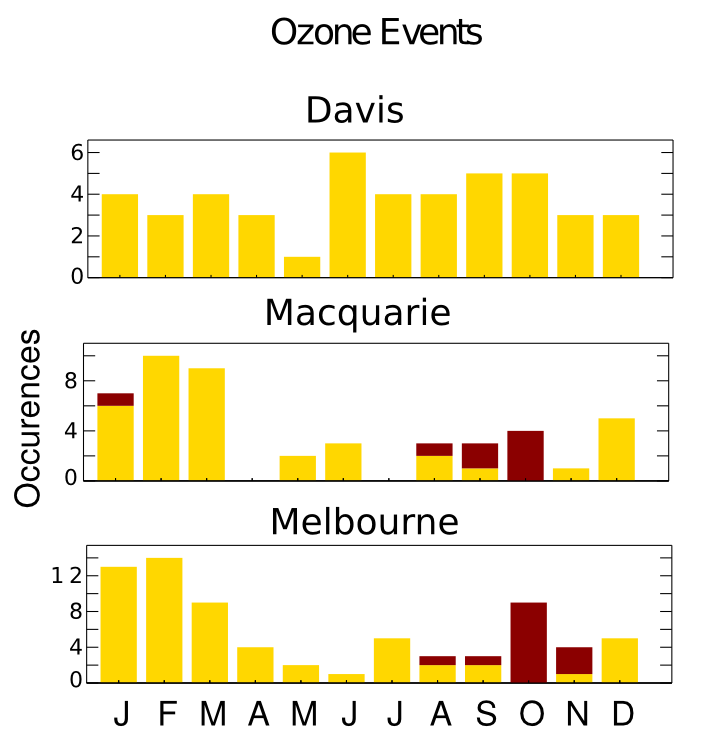
\includegraphics[width=1.0\columnwidth]{figures/Seasonality.png}
    \caption{The seasonality of STT events at Davis, Macquarie Island, and Melbourne.
    The events filtered out as possibly smoke plume influenced are indicated in red.}
    \label{fig:SummarySeasonality}
    \end{center}
  \end{figure}
  
  The frequency of STT events above Davis is relatively constant throughout the year, with a slight increase in events during antarctic winter.
  The slightly increased winter time frequency can be attributed to the increased frequency of sonde releases during the June to October months over Davis.
  It could be that events are non seasonal at Davis, or else that the sample of 45 detected events over 10 years is too small or sparse to clearly show any cycle.
  It is possible that summer events caused by upper troposphere turbulence are balanced out by the events caused by the polar front jet stream, which is strongest during antarctic winter.
  The polar front jet stream is a band of wind extending from the mid troposphere up to the lower stratosphere, which is generally active from winter to spring. 
  This vortex may be directly causing or impacting many of the STTs due to the lowered tropopause altitude which occurs south of the vortex edge (around 60$^\circ$~S).

  Figure \ref{fig:SummaryAltitudes} shows the altitudes of detected events, based on the peak of tropospheric ozone.
  STT event altitudes most commonly occur at 6 -- 10~km above Melbourne and below 8~km at Davis but are distributed more evenly at Macquarie Island. 
  Figure \ref{fig:SummaryTPDepths} shows the depths of detected events, based on the ozone peak's distance from the minimal determined tropopause.
  The majority of events occur within 3~km of the tropopause at both Melbourne and Macquarie Island, and within 2~km of the tropopause at Davis.
  
  For both Melbourne and Macquarie Island, the STT events which are unlikely to be fire-related occur mostly in summer and mostly during low pressure synoptic systems which can increase convection and upper tropospheric turbulence.

  \begin{figure}[!htbp]
    \begin{center}
    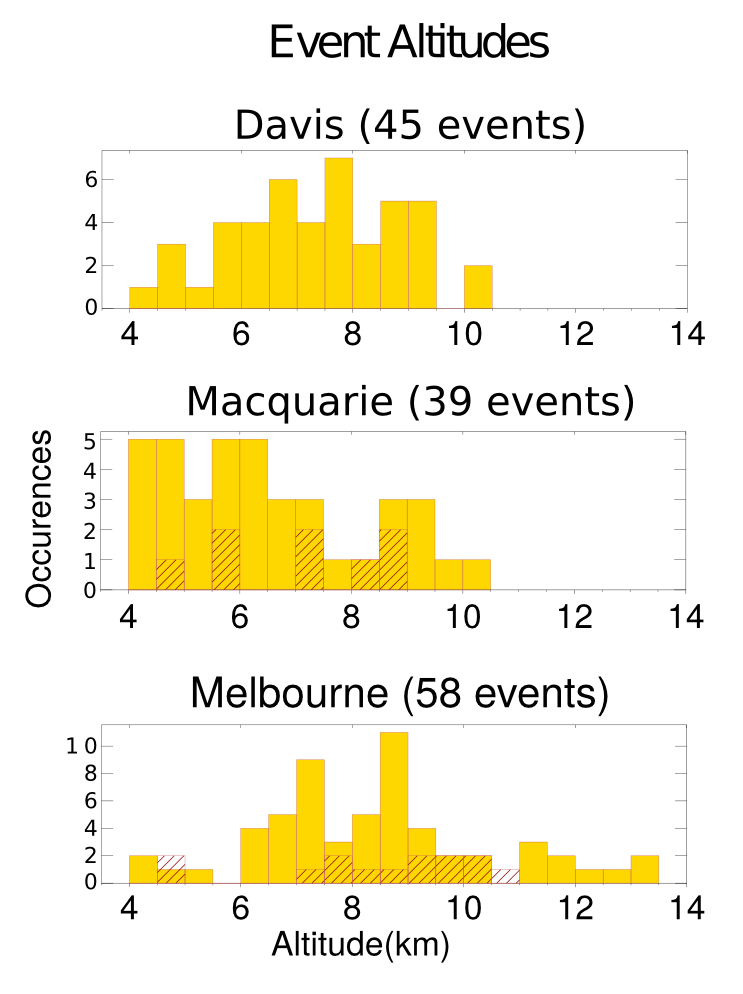
\includegraphics[width=0.99\columnwidth]{figures/Altitudes.png}
    \caption{The distribution of the ozone peak altitude for Davis, Macquarie Island, and Melbourne.
    This shows the altitude of detected events, based on the tropospheric ozone enhancement peak.
    Red diagonal lines show the removed smoke influenced event altitudes.}
    \label{fig:SummaryAltitudes}
    \end{center}
  \end{figure}

  \begin{figure}[!htbp]
    \begin{center}
    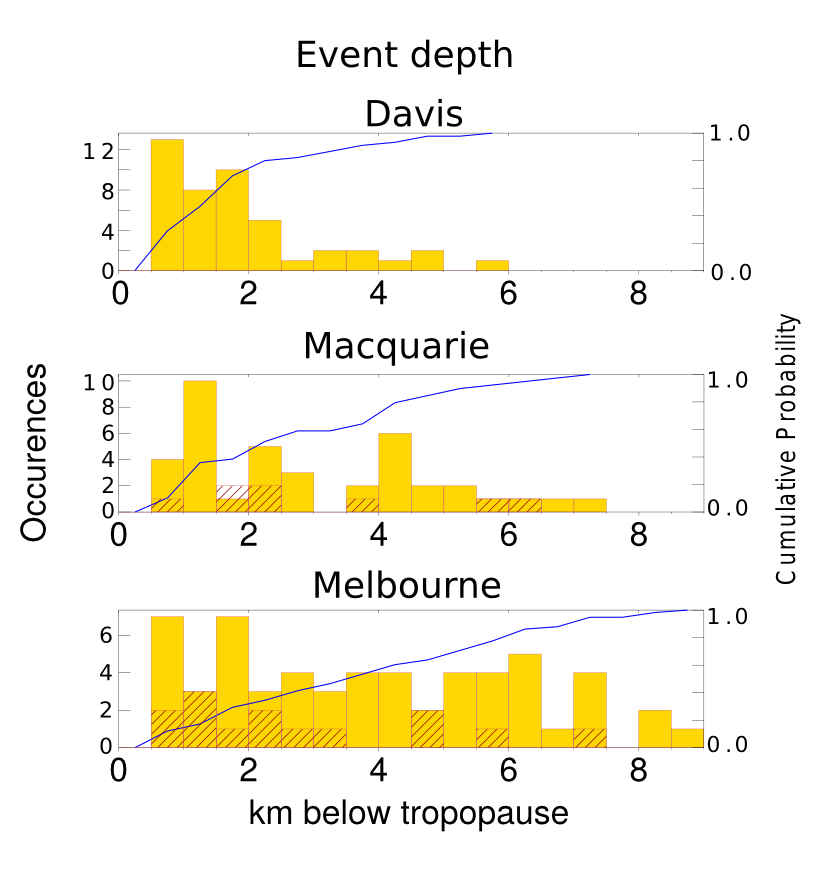
\includegraphics[width=0.99\columnwidth]{figures/TPDistance.png}
    \caption{The distance between the ozone peak and the tropopause, and the cumulative probability of these distances (blue line) for Davis, Macquarie Island, and Melbourne.
    This shows the depth of the event into the troposphere, starting from the tropopause.
    Red diagonal lines show the removed smoke-influenced event depths}
    \label{fig:SummaryTPDepths}
    \end{center}
  \end{figure}

\section{Comparison with GEOS-Chem}
  GEOS-Chem version 10.01 is a global chemical-transport model developed at Harvard \citep{Bey2001}, which includes transport, emission, deposition, chemical creation and destruction of ozone and 103 other trace gases throughout the troposphere.
  The stratospheric chemistry, including photolysis, is also modeled and stratosphere-troposphere coupling is calculated with the addition of the stratospheric unified chemistry extension \citep{Eastham2014}, which also includes a further 28 trace gases.
  GEOS-Chem values compared against the ozonesondes are based on a simulation using UCX from 2004-2013 exclusive, with 2004 used as a spinup year.
  Our GEOS-Chem run included a fix for properly reading Total Ozone Mapping Spectrometer (TOMS) satellite information.
  
  \begin{figure}[!htbp]
    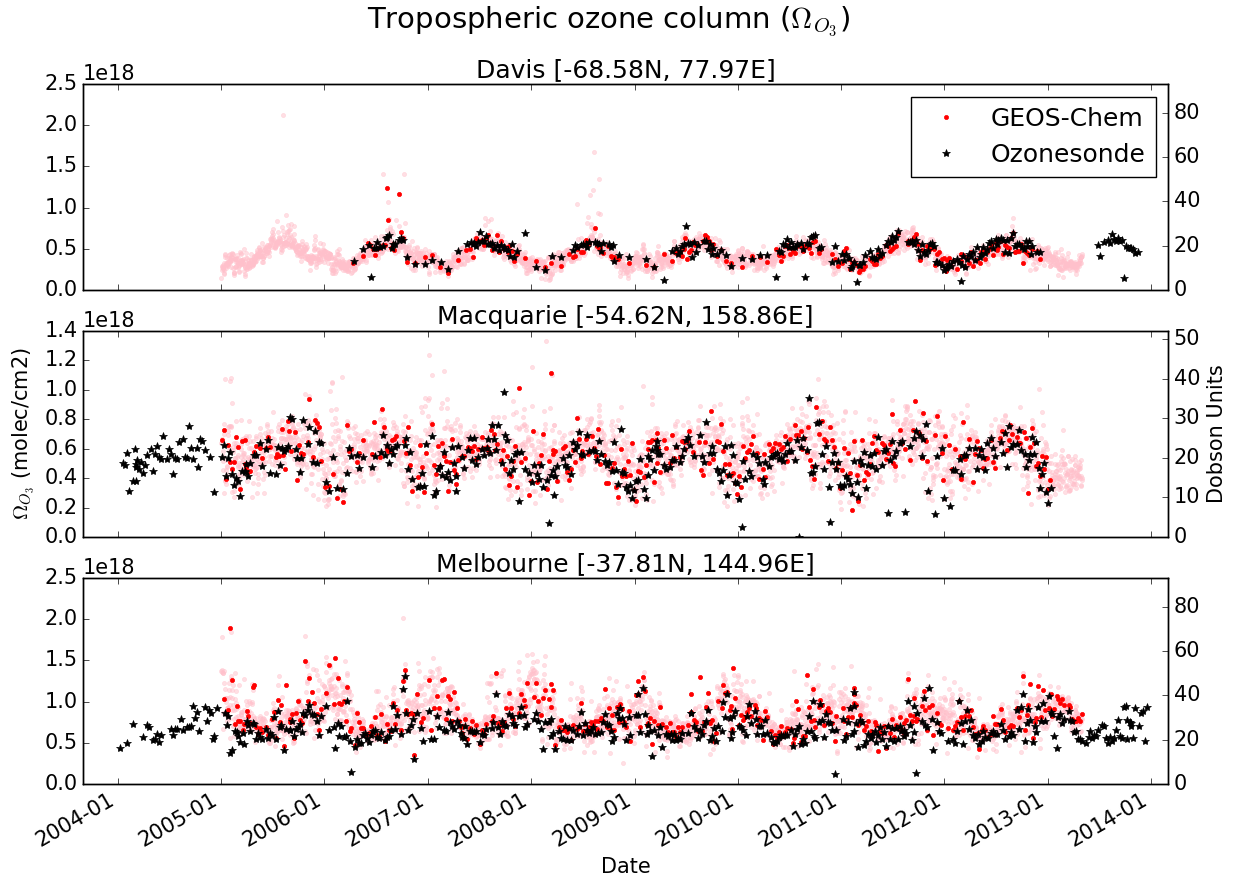
\includegraphics[width=\textwidth]{figures/StationSeries.png}
    \caption{Tropospheric ozone in molecules cm$^{-2}$ every six hours simulated by GEOS-Chem (blue) from January 1 2004 until December 31 2010. The ozonesonde calculated tropospheric ozone columns are shown as stars, each representing one measurement. (TODO: Update once fixed model run finishes)}
    \label{fig:StationSeriesGEOSChem}
  \end{figure}
  
  Figure \ref{fig:StationSeriesGEOSChem} shows the time series of tropospheric ozone column (TVC$_{O_3}$) in molecules cm$^{-2}$ from the GEOS-Chem simulation.
  Coplotted as stars are the measured tropospheric ozone columns calculated using the GPH and ozone partial pressure recorded by the ozone sondes.
  There is good aggreement between the modelled tropospheric ozone columns and the measurements, with matching seasonal cycles and magnitude.
  All three sites have a discernable yearly cycle, with Davis having the least spread as well as the greatest outliers.
  These outlying tropospheric ozone columns all occur during the July to September months.
  The seasonal maximum for Melbourne is in summer, with a minimum in winter, which is the opposite of both Macquarie and Davis.
  Both Macquarie Island and Melbourne have more variance in their tropospheric columns.
  For both sites the data is more spread out over the winter months.
  
  \begin{figure}[!htbp]
    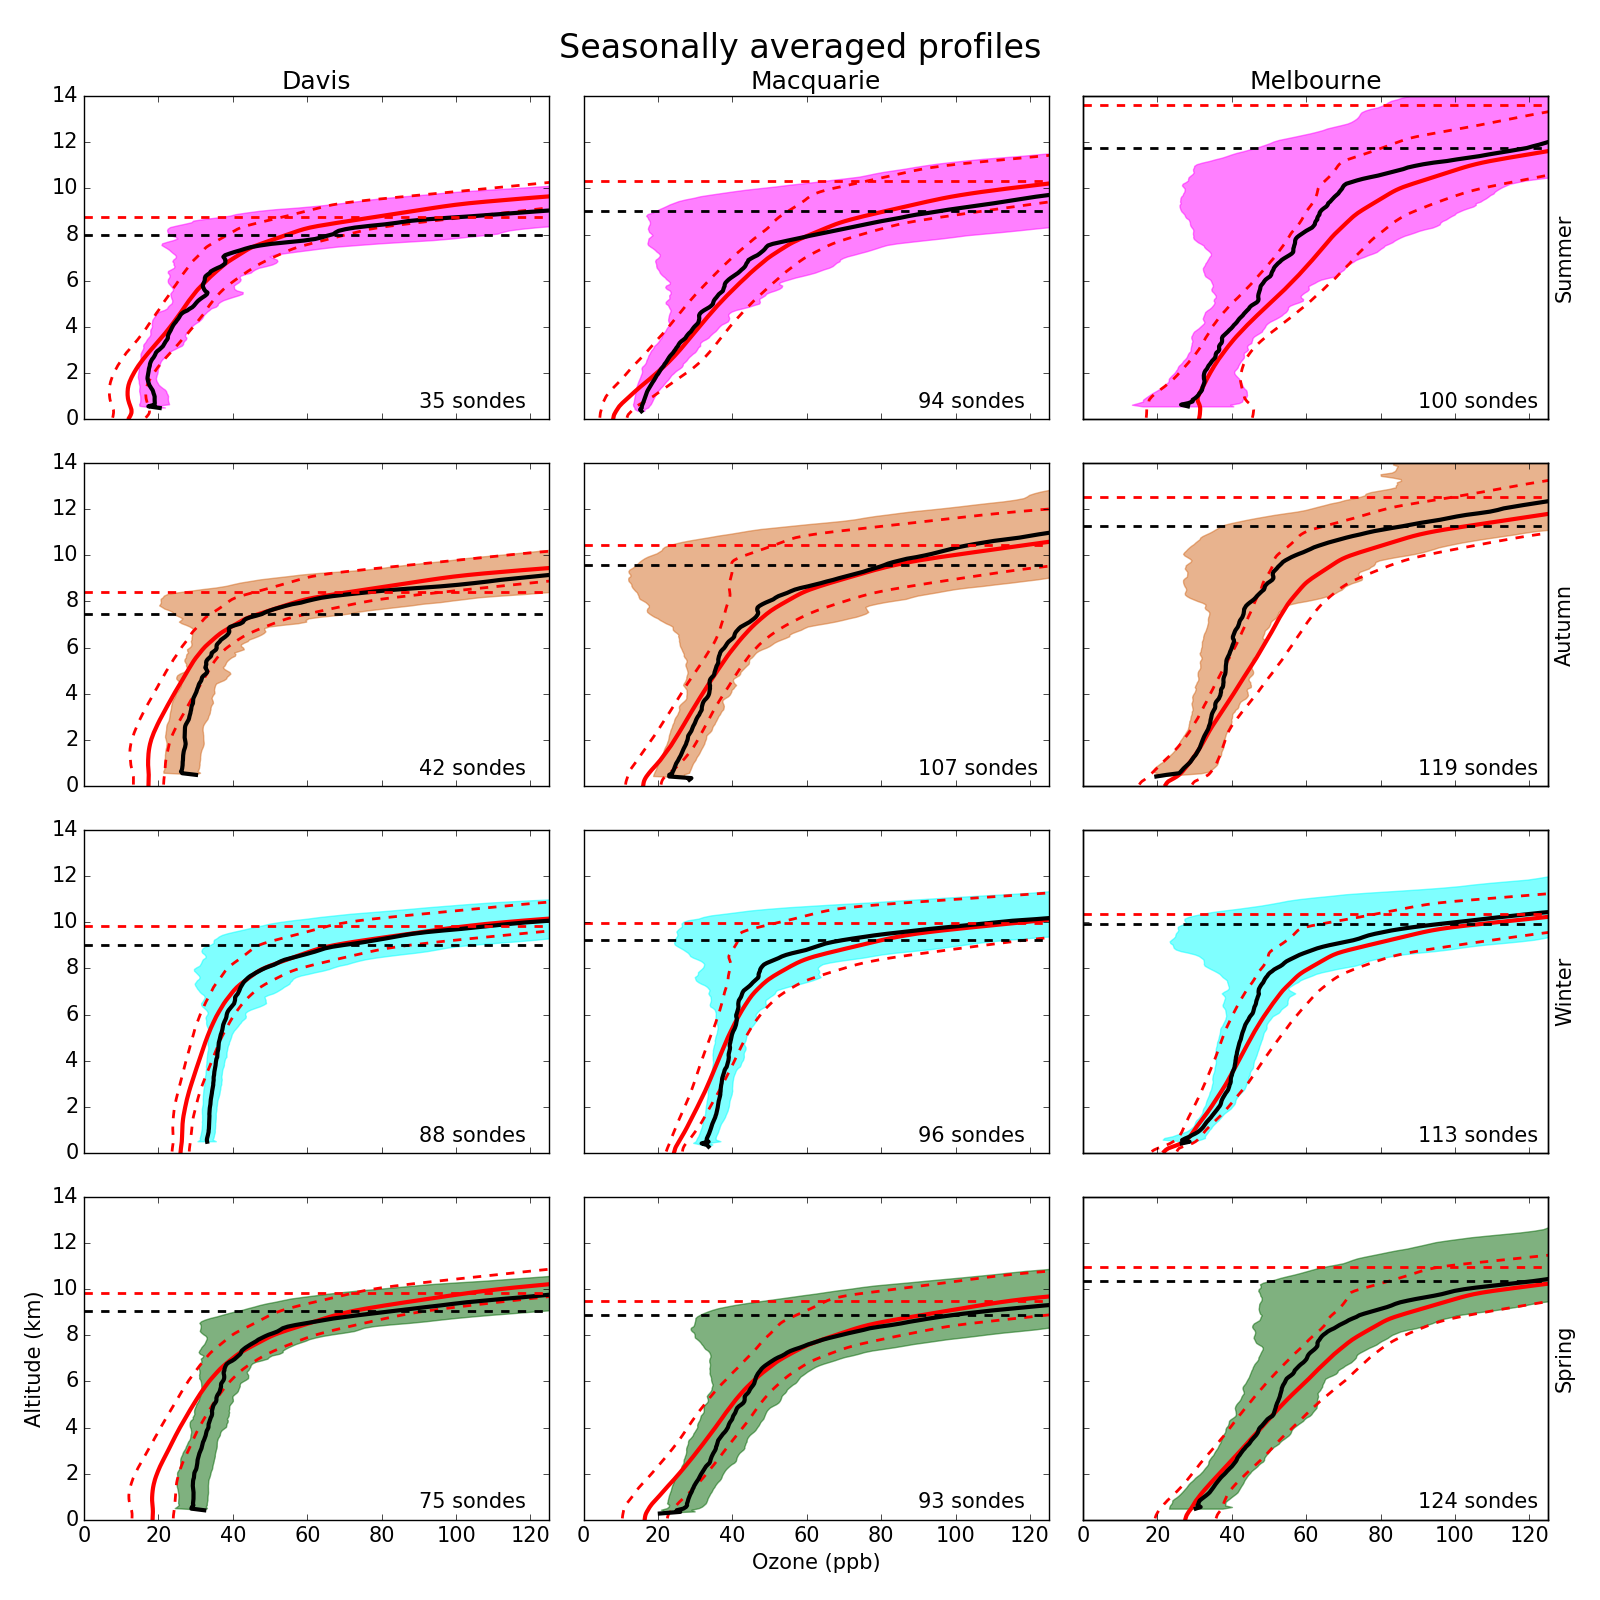
\includegraphics[width=\textwidth]{figures/seasonalprofiles00.png}
    \caption{Tropospheric ozone (ppb) over Davis, Macquarie, and Melbourne, seasonally averaged.
    GEOS-Chem simulated data averaged over January 2005 until December 2013 shown with black line, ozonesonde measurements shown with maroon line.
    The vertical axis is kilometres.
    Horizontal dotted line shows the mean tropopause height, shaded areas show one standard deviation.
    TODO: Update once fixed model run finishes.}
    \label{fig:GEOSChemSeasonalProfiles}
  \end{figure}
  
  Figure \ref{fig:GEOSChemSeasonalProfiles} shows the measured and simulated seasonal ozone profile for all three sites.
  Measurements are lower in the upper troposphere than the modeled profile, and more varied.
  The effect of pollution and mainland influence can be seen over Melbourne, mostly during the summer months (DJF), as the lower altitudes have increased ozone mean as well as more variance.
  Melbourne sondes show less ozone in the upper troposphere compared to the GEOS-Chem simulated profiles.
    
  
\section{Stratosphere to troposphere ozone flux from STT events}
  
  Based on the integrated ozone amount associated with each STT event (see section \ref{Section:CharacterisationOfSTTs}), we find a lower bound for the STT ozone flux over each of our three sites (fire influence excluded).
  This is a conservative lower bound as the algorithm ignores secondary ozone peaks which may also be transported down from the stratosphere, as well as ignoring potential ozone dispersion from the ozone peak.
  Figure \ref{fig:fluxsummary} shows the mean fraction of total tropospheric column ozone attributed to stratospheric ozone intrusions at each site, averaged over days when an STT event occurs.
  The mean fraction of tropospheric ozone attributed to STT events is 2--4\%, on individual days this value can exceed 10\% at Macquarie and Melbourne.
  Figure \ref{fig:fluxsummaryabs} shows the data in absolute terms, and indicates that the mean STT event impact is around $1$ to $2 \times 10^{18}$~molecules/cm$^2$.
  Our flux estimates are relatively insensitive to our biomass burning filter; including smoke-influenced days changes the mean flux by less than 0.25\% (5\% relative change).
  
  \begin{figure}[!htbp]
    \begin{center}
    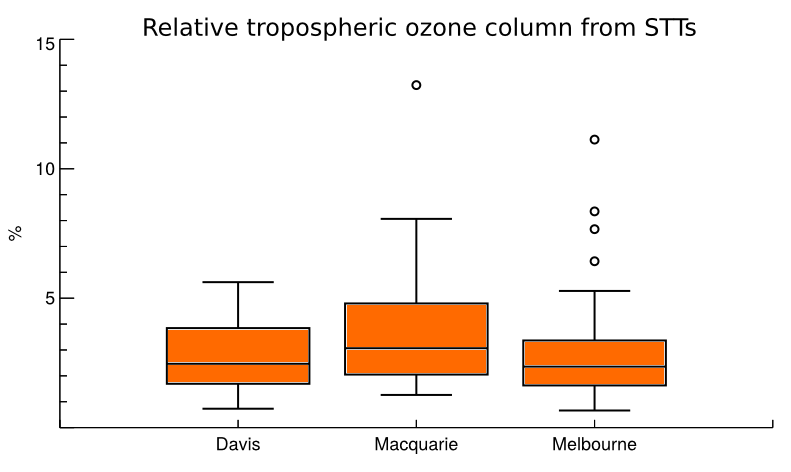
\includegraphics[width=0.8\columnwidth]{figures/flux_relative.png}
    \caption{Fraction of total tropospheric column ozone attributed to stratospheric air intrusions during STT events.}
    \label{fig:fluxsummary}
    \end{center}
  \end{figure}
  \begin{figure}[!htbp]
    \begin{center}
    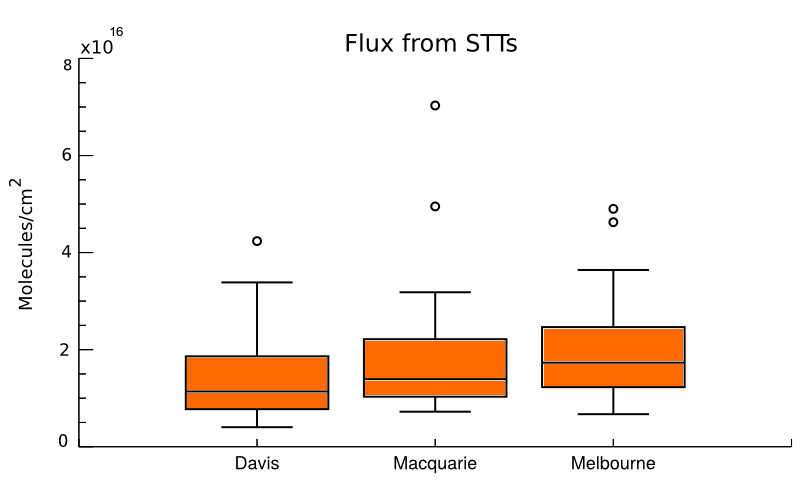
\includegraphics[width=0.8\columnwidth]{figures/flux_absolute.png}
    \caption{Tropospheric ozone attributed to stratospheric air intrusions during STT events.}
    \label{fig:fluxsummaryabs}
    \end{center}
  \end{figure}
  
  Extrapolating out over the Southern Ocean using our estimated enhanced tropospheric ozone, we can create a rough estimate of the STT effect on tropospheric ozone in this region.
  This is be done by multiplying the monthly likelihoods of STTs with the monthly tropospheric column ozone amounts multiplied by our mean flux fraction.
  Taking the monthly likelihood from our ozonesonde events count per sondes released during each month, and southern latitude tropospheric column ozone amount from GEOS-Chem, the total amount of ozone from STT events over the southern ocean is at least (TODO:update once fixed model is finished) $2.2\times10^{16}$ molecules cm$^{-2}$ yr$^{-1}$.
  Figure \ref{fig:SOExtrapolation} shows the seasonal STT contribution calculated this way, with l, f being the STT likelihood and fraction respectively.
    
  \begin{figure}[!htbp]
    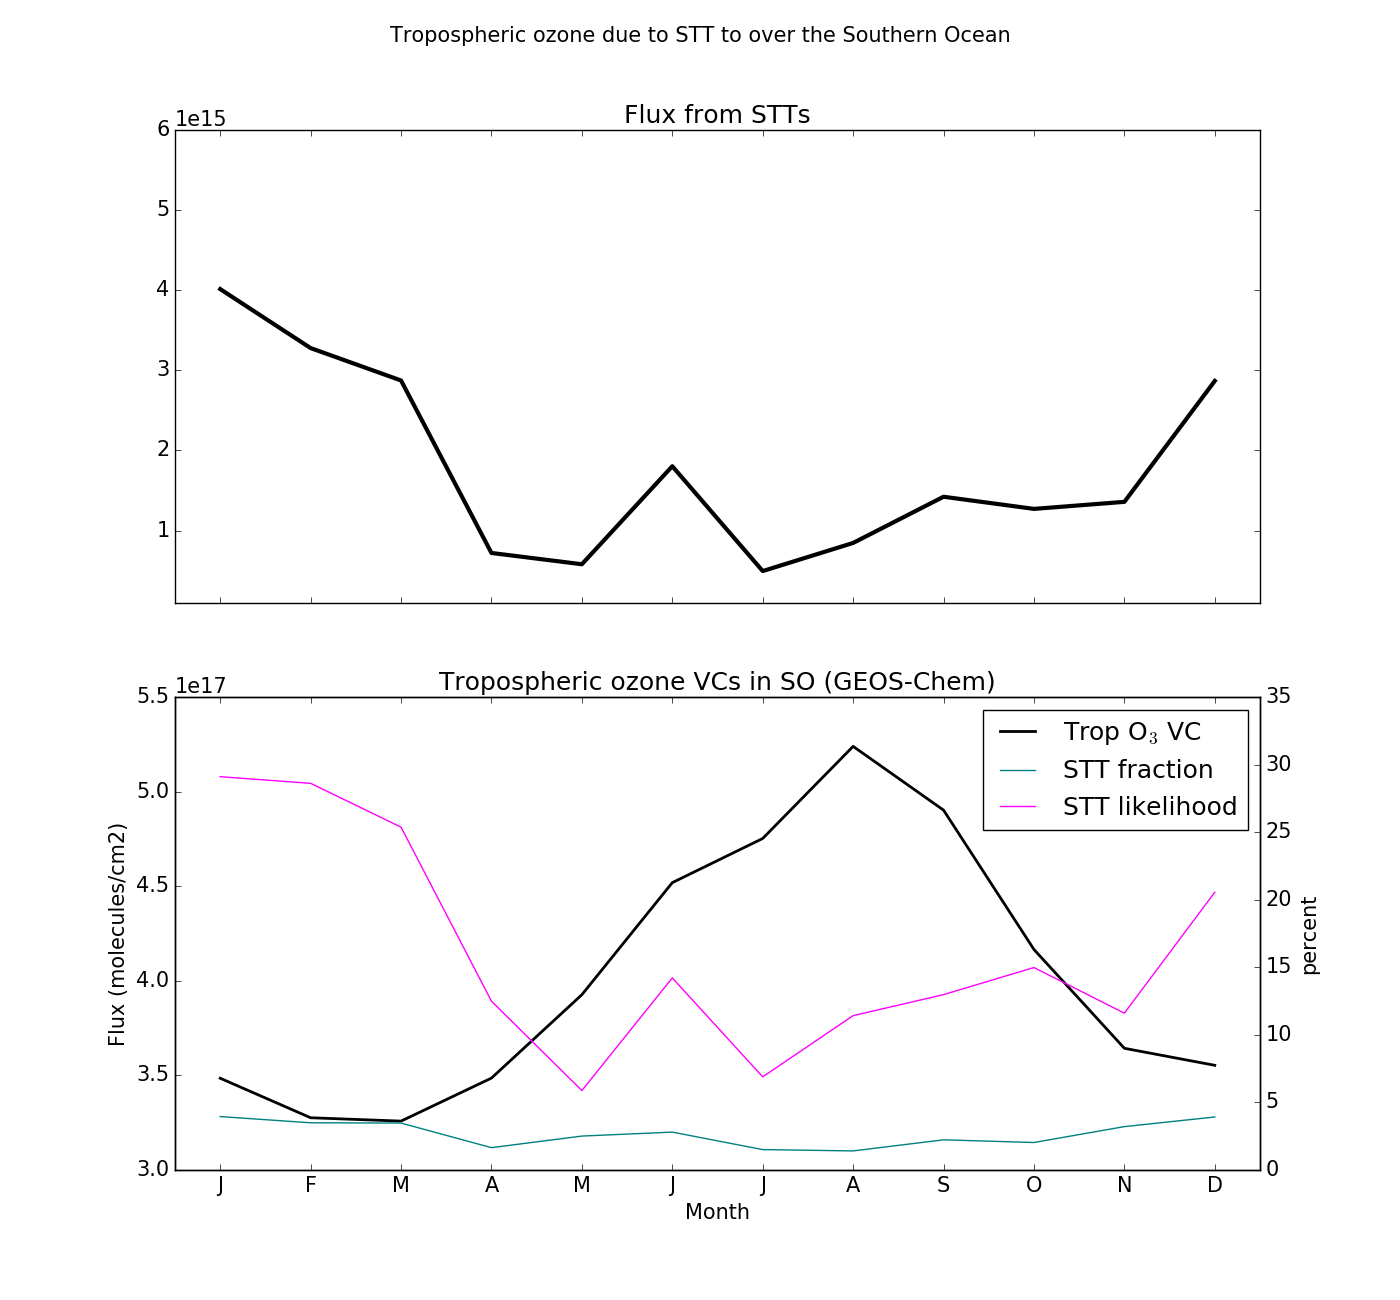
\includegraphics[width=\textwidth]{figures/SO_extrapolation.png}
    \caption{Top panel shows the estimated STT contribution to tropospheric ozone VC. Bottom panel shows the three factors multiplied together in order to produce the estimation. Units for l and f are on the right, while units for ozone VC amounts are on the left.}
    \label{fig:SOExtrapolation}
  \end{figure}
  

\section{Conclusion}
  
  Ozonesonde data in the Southern Hemisphere provides a satellite-independant quantification of STT ozone transport.
  The frequency and amount of ozone descending from the stratosphere into the troposphere can be estimated from the long time series of tropospheric ozone profiles.
  Using almost ten years of ozonesonde profiles over the southern high latitudes, a clear summer peak is seen for STT occurences at both 38$^{\circ}$S and 55$^{\circ}$S, although not at 69$^{\circ}$S.
  
  We use a band-pass filter to determine STT ozone transport events.
  The filter removes seasonal tropospheric ozone influences and allows clear detection of ozone-enhanced tongues of air in the troposphere.
  By setting empirical checks, ozonesonde vertical profiles can clearly show tropospheric ozone enhancement which is separated from the stratosphere.
  The cause of these ozone enhancements is examined through the use of satellite and reanalysis datasets on case studies above Melbourne.
  The major causes of STT events found over Melbourne are turbulent weather in the upper troposphere due to low pressure fronts and cut-off low pressure systems.
  
  Integration of the ozone enhancement along the altitude of the ozone profile allows a rough estimate of stratospheric transport for each event.
  Events typically cause a 3\% enhancement of the tropospheric ozone column.
  This is around $2*10^{11}$ molecules/cm$^3$ ozone enhancement over the southern high latitudes caused by STTs.
  
% This bibliography is created by mendeley automatically
%\bibliography{../../References/Ozone.bib}

% This one is a copy of the one above, feel free to edit it
\bibliography{bibliography/Ozone.bib}

\end{document}

